\chapter{Einleitung}\label{ch:einleitung}
Referenzen bis jetzt: \cite{Agarwal2006}, \cite{Ahlgren2012}, \cite{Bayardo2007}, \cite{Broder2004}, \cite{Byers2002}, \cite{Duerr2010}, \cite{Hellerstein1994}, \cite{Lehman1986}, \cite{Nafe2005}, \cite{Qiao2014}, \cite{Ruppel2014}, \cite{Sarwat2012}, \cite{Schnell2013}, \cite{Schoenfeld2014}, \cite{Shiraki2009}, \cite{Werner2015}, \cite{Yang2002}, \cite{Zhang2012}, \cite{Zhu2004}, \cite{Jannink1995}.
\section{Problembeschreibung}\label{sec:problem}
%\subsection{Referenz auf anderen Text}
%Es ist auch möglich auf andere Stellen im Text z.B. Kapitel \ref{subsec:sources} zu verweisen.
%\subsection{Tabellen}
%Es gibt schöne Möglichkeiten Tabellen einzubinden wie z.B. Tabelle \ref{tab:CommonParameterSettings}.
%\begin{center}
%\begin{table}[htbp]
%{\small
%\begin{center}
%\begin{tabular}[center]{lrlc}
%\toprule
%Parameter & Value & (Unit) & Available for Chord \\
%\midrule
%Query timeout & 10 & seconds & $\surd$ \\
%Republish timeout & 300 & seconds & $\surd$ \\ % explain this value...
%Stabilize timeout & 5 & seconds & $\surd$ \\
%Fix fingers timeout & 30 & seconds & $\surd$ \\
%Message timeout & 1 & second & $\surd$ \\
%Connect timeout & 10 & seconds & $\surd$ \\
%Ping superpeer timeout & 5 & seconds & $\times$ \\
%Cost-Optimality estimation timeout & 20 & seconds & $\times$ \\
%Significance for change in number of superpeers & 10 & percent & $\times$ \\
%Significance for change in estimations  & 10 & percent & $\times$ \\
%Number of permanent superpeers & 32 & nodes & $\times$ \\
%Mean number of peers & 1000 & nodes & $\surd$ \\
%Mean number of lookups per hour & 60 & queries & $\surd$ \\
%Mean number of shared InfoProfiles per node & 20 & & $\surd$ \\
%Identifier space & 16 & bits & $\surd$ \\
%Direct insertion acknowledgment & true & bool & $\times$ \\
%Direct query responses & true & bool & $\times$ \\
%Force query resolution & true & bool & $\surd$  \\
%\bottomrule
%\end{tabular}
%\end{center}
%} % end of tiny
%\caption[Simulation parameter settings]{Common simulation parameter settings.\label{tab:CommonParameterSettings}}
%\end{table}
%\end{center}
%
%\subsection{Bilder}
%Man kann sehr einfach Bilder einbinden so wie z.B. in Abbildung \ref{fig:pic0}.
%\begin{figure}[hpbt]
%  \centering
%  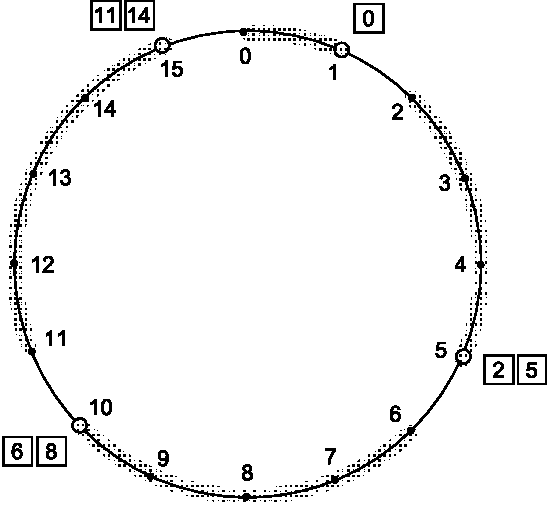
\includegraphics[width=0.4\textwidth]{pictures/pic0}\\
%  \caption[Example of a $4$-bit Chord identifier circle]{Example of a $4$-bit Chord identifier circle.
%  The responsibility ranges for each peer are accentuated in light gray}\label{fig:pic0}
%\end{figure}
%Es lassen sich auch mehrere Bilder nebeneinander platzieren wie z.B. in Abbildung
%\ref{fig:multipic} zu sehen ist.
%\begin{figure}[hpbt]
% \centering
%  %%----start of first subfigure----
%  \subfloat[FIFO size limited to 20 entries]{
%   \label{fig:multipic:a} %% label for first subfigure
%   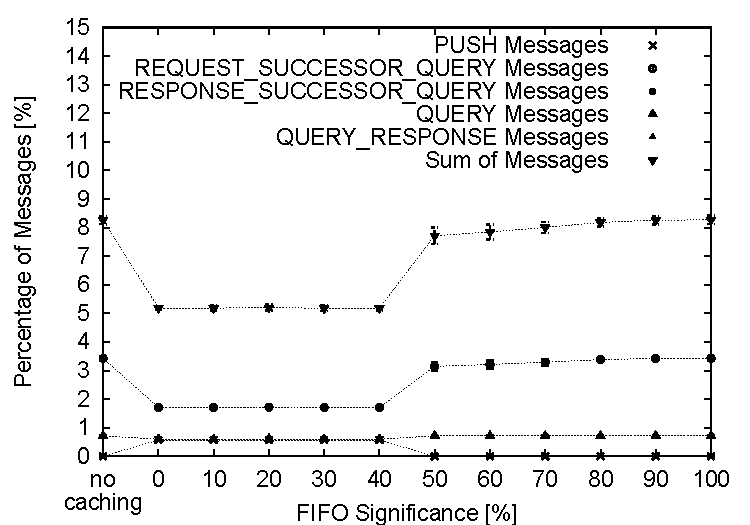
\includegraphics[width=0.48\linewidth]{pic1}}
%  \hspace{0.01\textwidth}
%  %%----start of second subfigure----
%  \subfloat[FIFO size limited to 30 entries]{
%   \label{fig:multipic:b} %% label for second subfigure
%   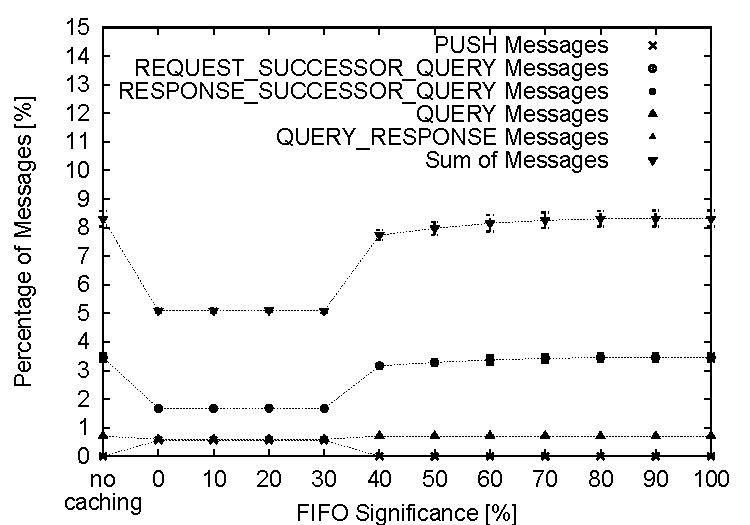
\includegraphics[width=0.48\linewidth]{pic2}}\\[0pt] % horizontal break
%  %%----start of third subfigure----
%  \subfloat[FIFO size limited to 40 entries]{
%   \label{fig:multipic:c} %% label for third subfigure
%   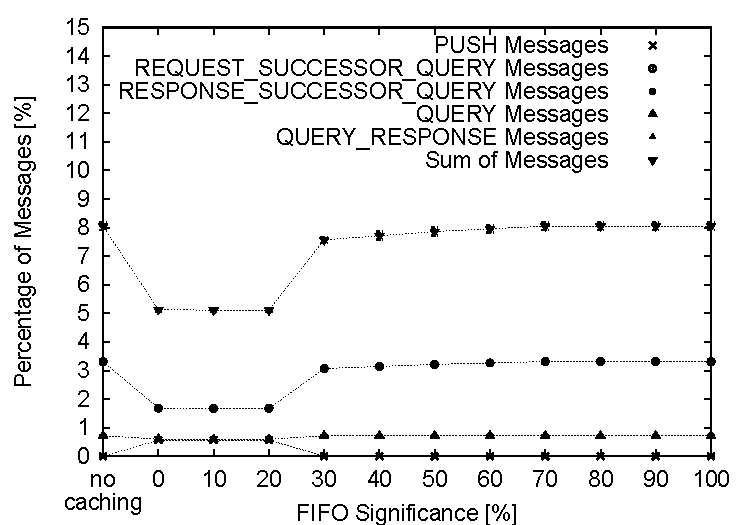
\includegraphics[width=0.48\linewidth]{pic3}}
%  \hspace{0.01\textwidth}
%  %%----start of fourth subfigure----
%  \subfloat[FIFO size limited to 50 entries]{
%   \label{fig:multipic:d} %% label for fourth subfigure
%   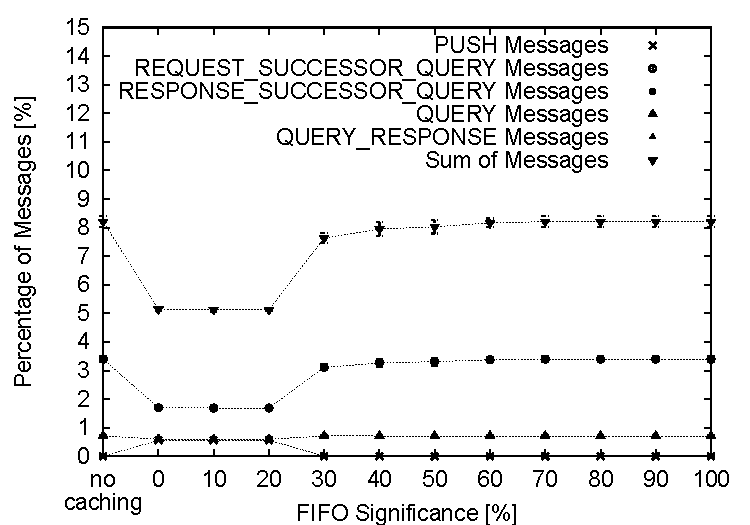
\includegraphics[width=0.48\linewidth]{pic4}}
% \caption[Observed message fractions and 95\% confidence intervals for Chord]{Observed message fractions and 95\% confidence intervals for Chord without the influence of churn. The FIFO capacity varies from 20 (\ref{fig:multipic:a}) -- 50 (\ref{fig:multipic:d}) entries (decadic steps).}
% \label{fig:multipic} %% label for entire figure
%\end{figure}
%
%\subsection{Programm Code}
%Eine elegante Möglichkeit, Programmtext einzubinden, lässt sich mit dem listings-Paket erreichen.
%Das \verb|HelloWorld| Programm aus Listing \ref{lst:hw} hat in Zeile \ref{line:hw3} übrigens einen Programmierfehler.
%\begin{lstlisting}[float=htp,caption=Hello World,label=lst:hw,language=Java, numbers=left, numberstyle=\tiny, stepnumber=2, numbersep=8pt, escapeinside={//@}{@//},backgroundcolor=\color{yellow},xleftmargin=3ex,xrightmargin=1ex]
%public class HelloWorld {
%    public static void main(String[] args) {
%        Syste.out.println("Hello, World"); //@\label{line:hw3}@//
%    }
%}
%\end{lstlisting}